\par El software evoluciona con el tiempo. Los requerimientos de negocio y producto se modifican conforme avanza el desarrollo, y los constantes cambios en el mercado hacen que sea muy difícil desarrollar un software en tiempo y forma. Para esto existen los modelos evolutivos, que están diseñados explícitamente para adaptarse a un producto evoluciona con el tiempo \cite{pressmanIngenieriaSoftwareEnfoque2013}. Los modelos evolutivos son iterativos. Están pensados para desarrollar versiones cada vez más completas del software
%
%
\subsection{Modelo en espiral}
\par El modelo en espiral se acopla la naturaleza iterativa de hacer prototipos con el aspecto más lineal y controlado de los métodos en cascada. El software se desarrolla en una serie de entregas evolutivas, donde en cada iteración se obtiene una versión más completa del software \cite{pressmanIngenieriaSoftwareEnfoque2013}.
\begin{figure}[H]
  \centering
  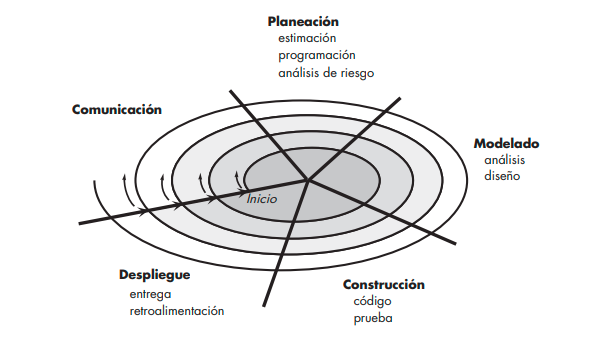
\includegraphics[scale=0.8]{image10.png}
  \caption{Modelo en espiral. Extraída de \cite{pressmanIngenieriaSoftwareEnfoque2013}.}
  \label{fig:x Modelo en espiral}
\end{figure}
\par El modelo en espiral se divide en un conjunto de actividades estructurales que se repiten en cada iteración. El primer circuito resulta en la especificación del producto. Las vueltas sucesivas se usan para desarrollar el prototipo y finalmente el resto de iteraciones son para crear el producto final [12].